% !TeX program = pdflatex
\documentclass[tikz,border=8pt]{standalone}
\usepackage{tikz}
\usetikzlibrary{positioning,arrows.meta}
\definecolor{FigureBlue}{HTML}{2563EB}\definecolor{FigureOrange}{HTML}{EA580C}
\begin{document}
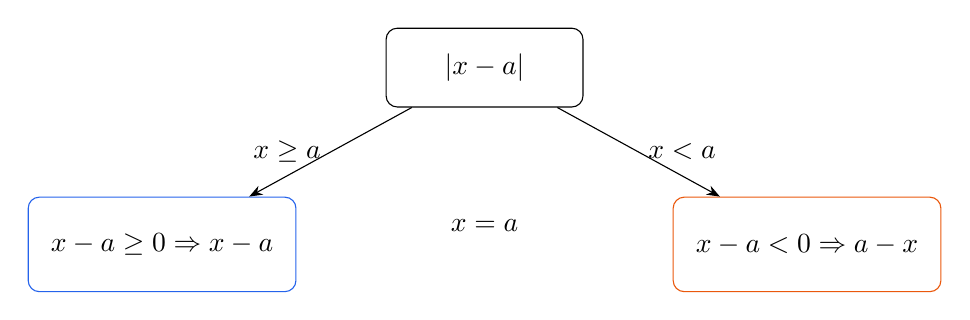
\begin{tikzpicture}[>=Stealth,node distance=16mm]
  \node[draw,rounded corners,minimum width=25mm,minimum height=10mm] (start) {$|x-a|$};
  \node[draw=FigureBlue,rounded corners,below left=of start,minimum width=34mm,minimum height=12mm] (pos) {$x-a\ge0\Rightarrow x-a$};
  \node[draw=FigureOrange,rounded corners,below right=of start,minimum width=34mm,minimum height=12mm] (neg) {$x-a<0\Rightarrow a-x$};
  \draw[->] (start)--(pos) node[midway,left] {$x\ge a$};
  \draw[->] (start)--(neg) node[midway,right] {$x<a$};
  \node[below=13mm of start] {$x=a$};
\end{tikzpicture}
\end{document}
